% Gabarit pandoc des corrigés publiés (brut et guidé). Contenu sans marque ni nom de site.
% Compilation : lualatex (latexmk -lualatex).
% Le Markdown reste la source unique : ne pas éditer ce fichier .tex à la main.
\documentclass[11pt,a4paper]{article}

% --- Moteur, polices (Latin Modern) et langue ---------------------------------
\usepackage{iftex}
\ifLuaTeX\else\errmessage{Ce document se compile avec lualatex}\fi
\usepackage{amsmath,amssymb,mathtools}
\usepackage{fontspec}
% mathrm=sym : \mathrm prend ses glyphes dans la police mathématique (ℓ, μ, Ω), comme KaTeX.
\usepackage[math-style=TeX,bold-style=TeX,mathrm=sym]{unicode-math}
% Repli pour les glyphes absents de Latin Modern (indices et exposants Unicode,
% flèches, filets des schémas en texte, symboles) : DejaVu, puis Latin Modern Math
% (ℓ, lettres mathématiques Unicode des légendes).
\directlua{
  luaotfload.add_fallback("repliTexte", {"DejaVuSerif:mode=harf;", "DejaVuSans:mode=harf;", "file:latinmodern-math.otf:mode=harf;"})
  luaotfload.add_fallback("repliMono", {"DejaVuSansMono:mode=harf;", "DejaVuSans:mode=harf;", "file:latinmodern-math.otf:mode=harf;"})
}
\setmainfont{Latin Modern Roman}[RawFeature={fallback=repliTexte}]
\setsansfont{Latin Modern Sans}[RawFeature={fallback=repliTexte}]
\setmonofont{Latin Modern Mono}[RawFeature={fallback=repliMono}]
\setmathfont{Latin Modern Math}
\usepackage[french]{babel}
\frenchsetup{SmallCapsFigTabCaptions=false}

% --- Mise en page --------------------------------------------------------------
\usepackage[a4paper,margin=2.2cm,headheight=14pt,footskip=1.2cm]{geometry}
\usepackage{microtype}
\setlength{\emergencystretch}{4em}
\tolerance=1500
\setlength{\parindent}{0pt}
\setlength{\parskip}{0.55\baselineskip plus 2pt minus 1pt}
\usepackage{xcolor}
% Gris nommés : babel-french rend « ! » actif dans le document.
\definecolor{gris2}{gray}{0.98}
\definecolor{gris3}{gray}{0.97}
\definecolor{gris5}{gray}{0.95}
\definecolor{gris35}{gray}{0.65}
\definecolor{gris40}{gray}{0.60}
\definecolor{gris45}{gray}{0.55}
\definecolor{gris50}{gray}{0.50}
\definecolor{gris55}{gray}{0.45}
\definecolor{gris60}{gray}{0.40}
\definecolor{gris65}{gray}{0.35}
\definecolor{gris70}{gray}{0.30}
\definecolor{gris80}{gray}{0.20}
\definecolor{gris85}{gray}{0.15}
\usepackage{graphicx}
\usepackage{float}
\usepackage{caption}
\captionsetup{font=small,labelformat=empty,justification=centering}
\usepackage{booktabs,longtable,array,multirow,calc}
\usepackage{siunitx}
\sisetup{locale=FR}
\usepackage[version=4]{mhchem}
\usepackage{listings}
\usepackage{fancyhdr}
\usepackage{lastpage}
\usepackage[most]{tcolorbox}
\usepackage{enumitem}
\setlist{nosep,leftmargin=*,topsep=2pt}
\usepackage[hidelinks,unicode]{hyperref}
\usepackage{bookmark}
\hypersetup{pdftitle={Mines-Ponts PSI — Maths 1 2026},pdfauthor={Rédigé par IA},pdfcreator={LaTeX},pdfsubject={Corrigé brut}}
\usepackage{xurl}

% --- Pandoc : listes, tableaux, figures ----------------------------------------
\providecommand{\passthrough}[1]{#1}
\providecommand{\tightlist}{\setlength{\itemsep}{0pt}\setlength{\parskip}{0pt}}

\makeatletter
\def\maxwidth{\ifdim\Gin@nat@width>\linewidth\linewidth\else\Gin@nat@width\fi}
\def\maxheight{\ifdim\Gin@nat@height>0.55\textheight 0.55\textheight\else\Gin@nat@height\fi}
\makeatother
\setkeys{Gin}{width=\maxwidth,height=\maxheight,keepaspectratio}
\setcounter{secnumdepth}{-\maxdimen}
\providecommand{\pandocbounded}[1]{#1}

% --- Code (listings) -----------------------------------------------------------
\lstset{
  basicstyle=\ttfamily\small,
  columns=fullflexible,
  keepspaces=true,
  breaklines=true,
  breakatwhitespace=false,
  postbreak=\mbox{\textcolor{gris50}{$\hookrightarrow$}\space},
  frame=single,
  rulecolor=\color{gris35},
  framesep=4pt,
  xleftmargin=5pt,xrightmargin=5pt,
  backgroundcolor=\color{gris3},
  keywordstyle=\bfseries,
  commentstyle=\color{gris65},
  stringstyle=\color{gris80},
  showstringspaces=false,
  tabsize=4,
  extendedchars=true,
  aboveskip=6pt,belowskip=6pt,
}

% --- Macros des corrigés (KaTeX ↔ LaTeX) ---------------------------------------
% Les corrigés sont écrits pour KaTeX : on définit ici ce que KaTeX connaît et
% que LaTeX n'a pas, sans jamais retoucher le Markdown.
\providecommand{\R}{\mathbb{R}}
\providecommand{\N}{\mathbb{N}}
\providecommand{\Z}{\mathbb{Z}}
\providecommand{\Q}{\mathbb{Q}}
\providecommand{\C}{\mathbb{C}}
\providecommand{\dd}{\mathrm{d}}
\providecommand{\llbracket}{\lBrack}
\providecommand{\rrbracket}{\rBrack}
\providecommand{\lBrace}{\lbrace}
\providecommand{\rBrace}{\rbrace}
\providecommand{\Box}{\square}
\providecommand{\Diamond}{\lozenge}
\providecommand{\varnothing}{\emptyset}
\providecommand{\argmax}{\operatorname*{arg\,max}}
\providecommand{\argmin}{\operatorname*{arg\,min}}
\renewcommand{\leq}{\leqslant}
\renewcommand{\geq}{\geqslant}

% Équation hors texte : réduite à la largeur de la ligne si elle déborde.
\newsavebox{\boiteequation}
\newcommand{\equationajustee}[1]{%
  \sbox{\boiteequation}{$\displaystyle #1$}%
  \ifdim\wd\boiteequation>\linewidth
    \[\resizebox{\linewidth}{!}{\usebox{\boiteequation}}\]%
  \else
    \[#1\]%
  \fi}

% --- Encadrés pédagogiques (sobres, lisibles en noir et blanc) -----------------
\tcbset{
  encadre/.style={
    enhanced,breakable,sharp corners,
    colback=white,colframe=gris55,
    boxrule=0.4pt,leftrule=2.2pt,
    left=6pt,right=6pt,top=3pt,bottom=3pt,
    before skip=6pt,after skip=6pt,
    fonttitle=\bfseries\small,coltitle=black,
    attach title to upper,after title={\quad},
    parbox=false,
  }
}
\newtcolorbox{indication}[1]{encadre,colframe=gris45,colback=gris2,title={Indication~#1}}
\newtcolorbox{methode}{encadre,colframe=gris70,title={Méthode}}
\newtcolorbox{piege}{encadre,colframe=gris85,boxrule=0.8pt,leftrule=2.2pt,title={Piège}}
\newtcolorbox{jury}{encadre,colframe=gris60,colback=gris5,title={Jury}}
\newtcolorbox{encadrenote}{encadre,colframe=gris40}

% --- Titres de section ---------------------------------------------------------
\usepackage{titlesec}
\titleformat{\section}{\Large\bfseries}{}{0pt}{}
\titleformat{\subsection}{\large\bfseries}{}{0pt}{}
\titleformat{\subsubsection}{\normalsize\bfseries}{}{0pt}{}
\titlespacing*{\section}{0pt}{14pt plus 4pt minus 2pt}{6pt}
\titlespacing*{\subsection}{0pt}{10pt plus 3pt minus 2pt}{4pt}
\titlespacing*{\subsubsection}{0pt}{8pt plus 2pt minus 2pt}{2pt}

% --- En-tête et pied de page ---------------------------------------------------
\pagestyle{fancy}
\fancyhf{}
\fancyhead[L]{\small\textsc{Corrigé brut} · Mines-Ponts PSI}
\fancyhead[R]{\small Maths 1 2026}
\fancyfoot[L]{\footnotesize Corrigé rédigé par IA, non officiel}
\fancyfoot[R]{\footnotesize \thepage\,/\,\pageref*{LastPage}}
\renewcommand{\headrulewidth}{0.4pt}
\renewcommand{\footrulewidth}{0pt}
\fancypagestyle{plain}{\fancyhf{}\fancyfoot[R]{\footnotesize \thepage\,/\,\pageref*{LastPage}}\fancyfoot[L]{\footnotesize Corrigé rédigé par IA, non officiel}\renewcommand{\headrulewidth}{0pt}}

\begin{document}
\thispagestyle{plain}
\begin{center}
  {\small\scshape Corrigé brut}\par\smallskip
  {\LARGE\bfseries Mines-Ponts PSI — Maths 1 2026\par}\medskip
  {\large Mines-Ponts · PSI · Maths 1 · 2026\par}
\end{center}
\vspace{2pt}\hrule\vspace{8pt}

\emph{Corrigé rédigé par IA, non officiel. Signalez toute erreur.}

Notations : \(\chi_A(X)=\det(XI_n-A)\) est unitaire de degré \(n\), de coefficient \(-\operatorname{tr}A\) sur \(X^{n-1}\).

On utilise la règle de produit des matrices élémentaires :

\equationajustee{E_{a,b}E_{c,d}=\delta_{b,c}E_{a,d}.}

\hypertarget{a-ruxe9duction-des-endomorphismes-de-carruxe9-nul}{%
\section{A --- Réduction des endomorphismes de carré nul}\label{a-ruxe9duction-des-endomorphismes-de-carruxe9-nul}}

\hypertarget{question-1}{%
\subsection{Question 1}\label{question-1}}

Soit \(\lambda\) une valeur propre de \(u\) et \(x\) un vecteur propre associé. Alors

\equationajustee{u^2(x)=\lambda^2x=0,}

et \(x\neq0\) impose \(\lambda=0\).

Réciproquement, le corps de base est \(\mathbb C\) : le polynôme \(\chi_u\), de degré \(n\geqslant1\), admet une racine, qui est valeur propre de \(u\). Donc

\equationajustee{\boxed{\operatorname{Sp}(u)=\{0\}.}}

Comme \(\chi_u\) est scindé sur \(\mathbb C\), \(u\) est trigonalisable. Sa trace est donc la somme de ses valeurs propres comptées avec leur multiplicité.

Ici \(\chi_u=X^n\) : la seule valeur propre \(0\) est de multiplicité \(n\), d'où

\equationajustee{\boxed{\operatorname{tr}(u)=n\times0=0.}}

\hypertarget{question-2}{%
\subsection{Question 2}\label{question-2}}

Si \(y=u(x)\in\operatorname{Im}u\), alors \(u(y)=u^2(x)=0\). Ainsi \(\operatorname{Im}u\subset\operatorname{Ker}u\).

Par le théorème du rang, \(\dim\operatorname{Ker}u=n-r\), donc \(r\leqslant n-r\), soit

\equationajustee{\boxed{r\leqslant\frac n2.}}

\hypertarget{question-3}{%
\subsection{Question 3}\label{question-3}}

En dimension finie, \(\operatorname{Ker}u\) admet un supplémentaire \(S\). Par le théorème du rang,

\equationajustee{\begin{aligned}
\dim S&=n-\dim\operatorname{Ker}u\\
&=n-(n-r)=r.
\end{aligned}}

Une base \((e_1,\dots,e_r)\) de \(S\) est une famille libre telle que \(\operatorname{Ker}u\oplus\operatorname{Vect}(e_1,\allowbreak \dots,\allowbreak e_r)=E\).

Soient \(\lambda_1,\dots,\lambda_r\) tels que \(\sum_i\lambda_iu(e_i)=0\). Le vecteur \(x=\sum_i\lambda_ie_i\) de \(S\) vérifie \(u(x)=0\).

Donc \(x\in\operatorname{Ker}u\cap S=\{0\}\), et la liberté de \((e_i)\) donne \(\lambda_1=\dots=\lambda_r=0\).

\textbf{La famille \((u(e_1),\dots,u(e_r))\) est libre.}

\hypertarget{question-4}{%
\subsection{Question 4}\label{question-4}}

Posons \(f_i=u(e_i)\). La famille \((f_1,\dots,f_r)\) est libre (Q3) et contenue dans \(\operatorname{Im}u\), donc dans \(\operatorname{Ker}u\) (Q2).

Par le théorème de la base incomplète, on la complète \textbf{par des vecteurs de \(\operatorname{Ker}u\)} en une base \((f_1,\dots,f_r,g_1,\dots,g_{n-2r})\) de \(\operatorname{Ker}u\). Ce noyau est de dimension \(n-r\), et \(n-2r\geqslant0\) par Q2.

Comme \(E=S\oplus\operatorname{Ker}u\), la concaténation

\equationajustee{\mathcal B=(e_1,\dots,e_r,f_1,\dots,f_r,g_1,\dots,g_{n-2r})}

est une base de \(E\). On a \(u(e_i)=f_i\), puis \(u(f_i)=0\) et \(u(g_j)=0\) (vecteurs du noyau). Donc

\equationajustee{\boxed{\operatorname{Mat}_{\mathcal B}(u)=\begin{pmatrix}0_r&0_r&(0)\\ I_r&0_r&(0)\\ (0)&(0)&0_{n-2r}\end{pmatrix}.}}

\begin{figure}[H]
\centering
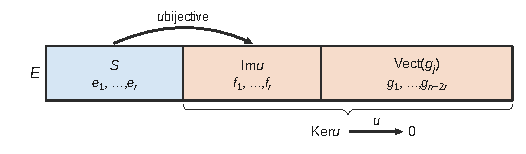
\includegraphics{figures/q4-structure-carre-nul.pdf}
\caption*{Figure 1 --- Base adaptée de Q4 : u envoie bijectivement S sur Im u
(f\_i = u(e\_i)) et annule Ker u = Im u ⊕ Vect(g\_j), les cases suivant
l'ordre de la base}
\end{figure}

\hypertarget{question-5}{%
\subsection{Question 5}\label{question-5}}

\emph{Existence} : \(m=r\) convient (Q4), et \(r>0\) car \(u\neq0\).

\emph{Unicité} : notons \(M_m\) la matrice de l'énoncé. Ses \(m\) premières colonnes sont les vecteurs de la base canonique d'indices \(m+1,\dots,2m\) ; les autres sont nulles. Donc \(\operatorname{rg}M_m=m\).

Si \(u\) est représenté par \(M_m\), le rang étant invariant par changement de base, \(m=\operatorname{rg}u=r\).

\equationajustee{\boxed{m=\operatorname{rg}(u)\ \text{est l'unique entier convenable.}}}

\hypertarget{b-somme-dun-nombre-arbitraire-dendomorphismes-de-carruxe9-nul}{%
\section{B --- Somme d'un nombre arbitraire d'endomorphismes de carré nul}\label{b-somme-dun-nombre-arbitraire-dendomorphismes-de-carruxe9-nul}}

\hypertarget{question-6}{%
\subsection{Question 6}\label{question-6}}

Par la règle de produit, \(E_{i,j}^2=\delta_{j,i}E_{i,j}\). C'est la matrice nulle si \(i\neq j\), et \(E_{i,i}\neq0\) si \(i=j\).

\textbf{Les \(E_{i,j}\) de carré nul sont exactement ceux avec \(i\neq j\).}

Soient \(i\neq j\). Les quatre matrices élémentaires qui composent \(F_{i,j}\) ne commutent pas entre elles : on ne peut donc pas utiliser d'identité remarquable. On développe le produit terme à terme, en multipliant \(F_{i,j}\) à gauche par chacun de ses termes :

\equationajustee{\begin{aligned}
E_{i,i}F_{i,j}&=E_{i,i}+E_{i,j},\\
-E_{j,j}F_{i,j}&=E_{j,j}+E_{j,i},\\
E_{i,j}F_{i,j}&=-E_{i,j}-E_{i,i},\\
-E_{j,i}F_{i,j}&=-E_{j,i}-E_{j,j}.
\end{aligned}}

En sommant ces quatre lignes :

\equationajustee{\boxed{(F_{i,j})^2=0_n\quad\text{pour tous }i\neq j.}}

Autre lecture : \(F_{i,j}\) annule les \(\varepsilon_k\) pour \(k\notin\{i,j\}\). Sur \(\operatorname{Vect}(\varepsilon_i,\varepsilon_j)\), il agit par la matrice \(\begin{pmatrix}1&1\\-1&-1\end{pmatrix}\), de carré nul.

\hypertarget{question-7}{%
\subsection{Question 7}\label{question-7}}

Soit \(A=(a_{i,j})\in\mathcal H_n\). Sur la base canonique,

\equationajustee{A=\sum_{i\neq j}a_{i,j}E_{i,j}+D,}

où \(D\) est la partie diagonale de \(A\) :

\equationajustee{D=\sum_{i=1}^na_{i,i}E_{i,i}.}

Comme \(\operatorname{tr}A=0\), on a \(a_{n,n}=-\sum_{i=1}^{n-1}a_{i,i}\). Par définition de \(F_{i,n}\), pour \(i\leqslant n-1\), on a aussi \(E_{i,i}-E_{n,n}=F_{i,n}-E_{i,n}+E_{n,i}\). D'où

\equationajustee{\begin{aligned}
D&=\sum_{i=1}^{n-1}a_{i,i}(E_{i,i}-E_{n,n})\\
&=\sum_{i=1}^{n-1}a_{i,i}\big(F_{i,n}-E_{i,n}+E_{n,i}\big).
\end{aligned}}

Donc

\equationajustee{\boxed{\begin{aligned}A={}&\sum_{i\neq j}a_{i,j}E_{i,j}+\sum_{i=1}^{n-1}a_{i,i}F_{i,n}\\&-\sum_{i=1}^{n-1}a_{i,i}E_{i,n}+\sum_{i=1}^{n-1}a_{i,i}E_{n,i}.\end{aligned}}}

C'est une combinaison linéaire de matrices \(E_{i,j}\) avec \(i\neq j\) (dans les deux dernières sommes, \(i\leqslant n-1\)) et de matrices \(F_{i,n}\) avec \(1\leqslant i\leqslant n-1\).

\hypertarget{question-8}{%
\subsection{Question 8}\label{question-8}}

On procède par double inclusion.

\(\subset\) : soit \(u=u_1+\dots+u_p\) avec \(u_k^2=0\) pour tout \(k\).

Chaque \(u_k\) est de trace nulle : par Q1 si \(u_k\neq0\), et c'est évident si \(u_k=0\).

Par linéarité de la trace, \(\operatorname{tr}u=0\).

\(\supset\) : soit \(u\in\mathcal H(E)\) et \(\mathcal B\) une base de \(E\). La matrice \(A=\operatorname{Mat}_{\mathcal B}(u)\) appartient à \(\mathcal H_n\).

Par Q7, on écrit \(A=\sum_{k=1}^N\lambda_kM_k\), où chaque \(M_k\) est un \(E_{i,j}\) (\(i\neq j\)) ou un \(F_{i,n}\).

Par Q6, \(M_k^2=0\), donc \((\lambda_kM_k)^2=\lambda_k^2M_k^2=0\).

L'application \(v\mapsto\operatorname{Mat}_{\mathcal B}(v)\) est un isomorphisme linéaire de \(\mathcal L(E)\) sur \(\mathcal M_n(\mathbb C)\) ; la matrice d'une composée est le produit des matrices.

Les endomorphismes \(u_k\) de matrices \(\lambda_kM_k\) vérifient donc \(u_k^2=0\), et \(u=u_1+\dots+u_N\in\Sigma_N\mathcal C(E)\).

\equationajustee{\boxed{\Sigma_\infty\mathcal C(E)=\mathcal H(E).}}

\hypertarget{c-somme-de-trois-endomorphismes-de-carruxe9-nul}{%
\section{C --- Somme de trois endomorphismes de carré nul}\label{c-somme-de-trois-endomorphismes-de-carruxe9-nul}}

\hypertarget{question-9}{%
\subsection{Question 9}\label{question-9}}

Soit \(n\geqslant5\) quelconque. Posons \(d=n-1\). Comme \(n>4\), on a \(4(n-1)>3n\), c'est-à-dire \(d>\frac{3n}4\).

Dans une base \((\varepsilon_1,\dots,\varepsilon_n)\) de \(E\), soit \(u\) l'endomorphisme de matrice

\equationajustee{\operatorname{diag}\big(1,\dots,1,-(n-1)\big).}

Alors \(\operatorname{tr}u=(n-1)-(n-1)=0\). La matrice de \(u-{\mathrm{id}}_E\) est \(\operatorname{diag}(0,\dots,0,-n)\), de rang \(1\).

Donc \(\dim\operatorname{Ker}(u-{\mathrm{id}}_E)=n-1=d\), et \(d\geqslant1\) : \(1\) est valeur propre, de sous-espace propre de dimension \(d>\frac{3n}4\).

\textbf{Un tel endomorphisme existe, pour tout \(n\geqslant5\).}

\hypertarget{question-10}{%
\subsection{Question 10}\label{question-10}}

\(\operatorname{Ker}w=\operatorname{Ker}(u-{\mathrm{id}}_E)\) est de dimension \(d\). Par le théorème du rang,

\equationajustee{\operatorname{rg}w=n-d<\frac n4.}

Les endomorphismes \(w\) et \(v\) ne commutent pas a priori. Comme \(v^2=0\) :

\equationajustee{\begin{aligned}
(w-v)^2&=w^2-wv-vw+v^2\\
&=w\circ(w-v)-v\circ w.
\end{aligned}}

On utilise \(\operatorname{rg}(a\circ b)\leqslant\min(\operatorname{rg}a,\allowbreak \operatorname{rg}b)\) (programme de première année) et \(\operatorname{rg}(a+b)\leqslant\operatorname{rg}a+\operatorname{rg}b\). Cette dernière inégalité vient de \(\operatorname{Im}(a+b)\subset\operatorname{Im}a+\operatorname{Im}b\) et de \(\dim(F+G)\leqslant\dim F+\dim G\) :

\equationajustee{\begin{aligned}
\operatorname{rg}\big((w-v)^2\big)&\leqslant\operatorname{rg}\big(w\circ(w-v)\big)+\operatorname{rg}(v\circ w)\\
&\leqslant\operatorname{rg}w+\operatorname{rg}w.
\end{aligned}}

Donc

\equationajustee{\boxed{\operatorname{rg}\big((w-v)^2\big)\leqslant2(n-d)<\frac n2.}}

\hypertarget{question-11}{%
\subsection{Question 11}\label{question-11}}

Soit \(N=\operatorname{Ker}(w-v)^2\). Par le théorème du rang et Q10, sa dimension vérifie

\equationajustee{q=n-\operatorname{rg}(w-v)^2>\frac n2.}

\emph{Stabilité.} \((w-v)^2\) est un polynôme en \(w-v\), donc commute avec \(w-v\). Pour \(x\in N\) :

\equationajustee{\begin{aligned}
(w-v)^2\big((w-v)(x)\big)&=(w-v)\big((w-v)^2(x)\big)\\
&=0.
\end{aligned}}

Ainsi \(N\) est stable par \(w-v\), donc par \(u-v=(w-v)+{\mathrm{id}}_E\).

\emph{Endomorphisme induit.} Soit \(s\) l'endomorphisme induit par \(w-v\) sur \(N\). Par définition de \(N\), \(s^2=0\).

Par l'argument de Q1 (valable aussi si \(s=0\)), \(\chi_s=X^q\). L'endomorphisme induit par \(u-v\) sur \(N\) est \(s+{\mathrm{id}}_N\), de polynôme caractéristique

\equationajustee{\det\big((X-1){\mathrm{id}}_N-s\big)=\chi_s(X-1)=(X-1)^q.}

\emph{Multiplicité.} Complétons une base de \(N\) en une base de \(E\). La matrice de \(u-v\) y est \(\begin{pmatrix}S&\ast\\0&T\end{pmatrix}\), avec \(\chi_S=(X-1)^q\). Par le déterminant triangulaire par blocs,

\equationajustee{\chi_{u-v}=(X-1)^q\chi_T.}

Ainsi

\equationajustee{\boxed{1\ \text{est valeur propre de }u-v\ \text{de \text{multiplicité}}\ \geqslant q=n-\operatorname{rg}\big((w-v)^2\big)\ (\geqslant1).}}

\hypertarget{question-12}{%
\subsection{Question 12}\label{question-12}}

Posons \(a=u-v\) et notons \(\mu_\lambda\) la multiplicité de \(\lambda\) comme racine de \(\chi_a\). Par Q10 et Q11,

\equationajustee{\mu_1\geqslant n-\operatorname{rg}(w-v)^2>\frac n2.}

Si \(-a=\varphi a\varphi^{-1}\), alors \(a\) et \(-a\) sont semblables, donc \(\chi_{-a}=\chi_a\). Or

\equationajustee{\begin{aligned}
\chi_{-a}(X)&=\det(X\,\mathrm{id}+a)\\
&=(-1)^n\det\big((-X)\mathrm{id}-a\big)\\
&=(-1)^n\chi_a(-X).
\end{aligned}}

Écrivons \(\chi_a=(X-1)^{\mu_1}Q\) avec \(Q(1)\neq0\). Alors

\equationajustee{\begin{aligned}
\chi_a(X)&=(-1)^n\chi_a(-X)\\
&=(-1)^{n+\mu_1}(X+1)^{\mu_1}Q(-X),
\end{aligned}}

et \(Q(-X)\) ne s'annule pas en \(-1\). Donc \(\mu_{-1}=\mu_1\), et

\equationajustee{\boxed{1\ \text{et}\ -1\ \text{sont valeurs propres de }u-v\ \text{de \text{multiplicités}}\ \mu_1=\mu_{-1}>\frac n2.}}

\hypertarget{question-13}{%
\subsection{Question 13}\label{question-13}}

Raisonnons par l'absurde : supposons \(u=v_1+v_2+v_3\) avec \(v_k\in\mathcal C(E)\). Posons \(v=v_3\), élément de \(\mathcal C(E)\), de sorte que Q10 à Q12 s'appliquent.

Alors \(u-v=v_1+v_2\in\Sigma_2\mathcal C(E)\). Le théorème de Wang et Wu fournit \(\varphi\in GL(E)\) tel que \(-(u-v)=\varphi\circ(u-v)\circ\varphi^{-1}\).

Par Q12, les racines distinctes \(1\) et \(-1\) de \(\chi_{u-v}\) ont des multiplicités \(\mu_1\) et \(\mu_{-1}\) toutes deux \(>\frac n2\).

Or la somme des multiplicités des racines de \(\chi_{u-v}\) est au plus son degré \(n\) :

\equationajustee{n\geqslant\mu_1+\mu_{-1}>n,}

ce qui est absurde. Donc

\equationajustee{\boxed{u\notin\Sigma_3\mathcal C(E),}}

alors que \(u\in\Sigma_\infty\mathcal C(E)\) par Q8, puisque \(\operatorname{tr}u=0\).

\hypertarget{d-intermuxe8de-matrices-de-hessenberg}{%
\section{D --- Intermède : matrices de Hessenberg}\label{d-intermuxe8de-matrices-de-hessenberg}}

\hypertarget{question-14}{%
\subsection{Question 14}\label{question-14}}

Notons \(M(x)=xI_n-A=(m_{i,j})\). On a \(m_{i,j}=0\) si \(i>j+1\), et \(m_{i+1,i}=-a_{i+1,i}\neq0\).

La matrice \(\widetilde{M(x)}^{(k,n)}\) a ses lignes indexées par \(\{1,\dots,n\}\setminus\{k\}\) et ses colonnes par \(\{1,\dots,n-1\}\). Découpons les lignes en \(\{1,\dots,k-1\}\cup\{k+1,\dots,n\}\) et les colonnes en \(\{1,\dots,k-1\}\cup\{k,\dots,n-1\}\) :

\begin{itemize}
\tightlist
\item
  bloc (lignes \(\geqslant k+1\), colonnes \(\leqslant k-1\)) : \(i-j\geqslant2\), donc il est nul ;
\item
  bloc (lignes \(\leqslant k-1\), colonnes \(\leqslant k-1\)) : c'est \(xI_{k-1}-A_{k-1}\), où \(A_{k-1}=(a_{i,j})_{1\leqslant i,j\leqslant k-1}\) ;
\item
  bloc (lignes \(k+p\), colonnes \(k-1+q\), avec \(1\leqslant p,q\leqslant n-k\)) : il est nul si \(p>q\), car alors \((k+p)-(k-1+q)\geqslant2\). Il est donc triangulaire supérieur, de diagonale \(m_{k+p,k+p-1}=-a_{k+p,k+p-1}\).
\end{itemize}

Le déterminant d'une matrice triangulaire par blocs est le produit des déterminants des blocs diagonaux :

\equationajustee{\det\Big(\widetilde{(xI_n-A)}^{(k,n)}\Big)=\Big(\prod_{i=k}^{n-1}(-a_{i+1,i})\Big)\chi_{A_{k-1}}(x).}

On convient que \(\chi_{A_0}=1\) pour \(k=1\), et qu'un produit vide vaut \(1\) pour \(k=n\). Le polynôme

\equationajustee{P_k=\Big(\prod_{i=k}^{n-1}(-a_{i+1,i})\Big)\chi_{A_{k-1}}}

convient. Il est de degré \(k-1\) : \(\chi_{A_{k-1}}\) est unitaire de degré \(k-1\), et le produit est non nul par régularité.

Il est unique : deux polynômes égaux en tout point de \(\mathbb C\), ensemble infini, sont égaux.

\equationajustee{\boxed{\deg P_k=k-1}}

\equationajustee{\boxed{\text{coefficient dominant de }P_k\ :\ (-1)^{n-k}\prod_{i=k}^{n-1}a_{i+1,i}.}}

\hypertarget{question-15}{%
\subsection{Question 15}\label{question-15}}

Soit \(C={}^t(c_1,\dots,c_{n-1})\) et \(\gamma={}^t(c_1,\dots,c_{n-1},0)\). Les matrices \(xI_n-(A+E_C)\) et \(xI_n-A\) ne diffèrent que par la dernière colonne : on passe de la seconde à la première en retranchant \(\gamma\) à cette colonne.

Par linéarité du déterminant par rapport à la dernière colonne, \(\chi_{A+E_C}(x)=\chi_A(x)-\det D(x)\), où \(D(x)\) a les \(n-1\) premières colonnes de \(xI_n-A\) et \(\gamma\) pour dernière colonne.

On développe \(\det D(x)\) selon sa dernière colonne. Supprimer la ligne \(k\) et cette colonne redonne les mineurs de \(xI_n-A\), d'où

\equationajustee{\chi_{A+E_C}=\chi_A-\sum_{k=1}^{n-1}(-1)^{k+n}c_kP_k.}

Notons \((\ast)\) cette relation.

Soit \(P\) unitaire de degré \(n\), de coefficient \(-\operatorname{tr}A\) sur \(X^{n-1}\).

Les polynômes \(\chi_A\) et \(P\) ont les mêmes coefficients en \(X^n\) et en \(X^{n-1}\).

Donc \(R=\chi_A-P\) appartient à \(\mathbb C_{n-2}[X]\). Par \((\ast)\), l'égalité \(\chi_{A+E_C}=P\) équivaut à

\equationajustee{\sum_{k=1}^{n-1}(-1)^{k+n}c_kP_k=R.}

Les polynômes \(P_1,\dots,P_{n-1}\) sont de degrés \(0,1,\dots,n-2\) (Q14). Cette famille échelonnée en degré est libre. Elle a \(n-1=\dim\mathbb C_{n-2}[X]\) éléments, c'est donc une base de \(\mathbb C_{n-2}[X]\).

Notons \((\mu_k)\) les coordonnées de \(R\) dans cette base. La condition équivaut à \(c_k=(-1)^{k+n}\mu_k\) pour tout \(k\).

\equationajustee{\boxed{\text{Il existe un unique }C\in\mathbb C^{n-1}\text{ tel que }\chi_{A+E_C}=P.}}

\hypertarget{question-16}{%
\subsection{Question 16}\label{question-16}}

\(J_n\) est de Hessenberg régulière et de trace nulle. Le polynôme \(X^n\) est unitaire, de coefficient \(0=-\operatorname{tr}J_n\) sur \(X^{n-1}\) : Q15 donne l'existence et l'unicité de \(C\).

Or \(xI_n-J_n\) est triangulaire inférieure de diagonale \(x\), donc \(\chi_{J_n}=X^n\) : le vecteur nul convient. Par unicité,

\equationajustee{\boxed{C=0.}}

\hypertarget{question-17}{%
\subsection{Question 17}\label{question-17}}

Soit \(A=(a_{i,j})\) la matrice de \(u\). Pour \(j\leqslant n-1\), \(u(e_j)\in\operatorname{Vect}(e_1,\dots,e_{j+1})\), avec la coordonnée \(a_{j+1,j}\) sur \(e_{j+1}\).

Montrons par récurrence sur \(k\in[\![0,n-1]\!]\) la propriété suivante : \(u^k(e_1)\in\operatorname{Vect}(e_1,\dots,e_{k+1})\), avec la coordonnée \(\pi_k=\prod_{i=1}^ka_{i+1,i}\) sur \(e_{k+1}\).

Elle est vraie pour \(k=0\), avec \(\pi_0=1\). Supposons-la vraie au rang \(k\leqslant n-2\), et écrivons \(u^k(e_1)=\sum_{i\leqslant k+1}\lambda_ie_i\), avec \(\lambda_{k+1}=\pi_k\).

Alors \(u^{k+1}(e_1)=\sum_{i\leqslant k+1}\lambda_iu(e_i)\) appartient à \(\operatorname{Vect}(e_1,\dots,e_{k+2})\). Seul le terme \(\lambda_{k+1}u(e_{k+1})\) a une composante sur \(e_{k+2}\), égale à \(\pi_ka_{k+2,k+1}=\pi_{k+1}\).

La matrice de \((u^k(e_1))_{0\leqslant k\leqslant n-1}\) dans \((e_1,\dots,e_n)\) est donc triangulaire supérieure, de diagonale \(\pi_0,\dots,\pi_{n-1}\). Ces coefficients sont non nuls par régularité : la matrice est inversible.

\equationajustee{\boxed{(u^k(e_1))_{0\leqslant k\leqslant n-1}\ \text{est une base de }E.}}

\hypertarget{question-18}{%
\subsection{Question 18}\label{question-18}}

Soit \(u\) l'endomorphisme de \(\mathbb C^n\) canoniquement associé à \(A\), et \((e_1,\dots,e_n)\) la base canonique.

\emph{\(u^n=0\).} Le polynôme \(\chi_A=X^n\) est scindé : \(A=QTQ^{-1}\) avec \(T\) triangulaire supérieure, de diagonale formée des valeurs propres, toutes nulles.

Avec \(G_k=\operatorname{Vect}(\varepsilon_1,\dots,\varepsilon_k)\) et \(G_0=\{0\}\), on a \(TG_k\subset G_{k-1}\). Donc \(T^n=0\), puis \(A^n=QT^nQ^{-1}=0\). C'est aussi la conclusion directe du théorème de Cayley--Hamilton.

\emph{Conclusion.} Par Q17 appliquée dans la base canonique, la famille \((f_0,\dots,f_{n-1})=(e_1,u(e_1),\dots,u^{n-1}(e_1))\) est une base de \(\mathbb C^n\).

On a \(u(f_k)=f_{k+1}\) pour \(k\leqslant n-2\), et \(u(f_{n-1})=u^n(e_1)=0\). La matrice de \(u\) dans cette base est \(J_n\).

\equationajustee{\boxed{A\ \text{est semblable \text{à}}\ J_n.}}

\hypertarget{e-somme-de-quatre-endomorphismes-de-carruxe9-nul}{%
\section{E --- Somme de quatre endomorphismes de carré nul}\label{e-somme-de-quatre-endomorphismes-de-carruxe9-nul}}

\hypertarget{question-19}{%
\subsection{Question 19}\label{question-19}}

\emph{\(A+V\) est de Hessenberg.} Soit \(i>j+1\). Alors \(i>j\) et \((i,j)\neq(n,n-1)\), donc \(a_{i,j}=0\) ; de plus \(V_{i,j}=0\).

\emph{\(A+V\) est régulière.} Pour \(i\leqslant n-2\), \((A+V)_{i+1,i}=0+1=1\). Enfin, la dernière ligne de \(V\) étant nulle, \((A+V)_{n,n-1}=a_{n,n-1}\neq0\).

\emph{Choix de \(C_0\).} On a \(\operatorname{tr}(A+V)=\operatorname{tr}A=0\).

Le polynôme \(X^n\) est unitaire, de coefficient \(0=-\operatorname{tr}(A+V)\) sur \(X^{n-1}\). Q15 fournit \(C_0\in\mathbb C^{n-1}\) tel que \(\chi_{A+V+E_{C_0}}=X^n\).

\emph{Conclusion.} \(E_{C_0}\) n'a de coefficients non nuls qu'en positions \((i,n)\) avec \(i\leqslant n-1\), strictement au-dessus de la diagonale. Donc \(A+V+E_{C_0}\) reste de Hessenberg régulière, de polynôme caractéristique \(X^n\). Par Q18 :

\equationajustee{\boxed{A+V+E_{C_0}\ \text{est semblable \text{à}}\ J_n.}}

\hypertarget{question-20}{%
\subsection{Question 20}\label{question-20}}

On a \(J_n=\sum_{i=1}^{n-1}E_{i+1,i}\). Posons

\equationajustee{B_1=\sum_{\substack{1\leqslant i\leqslant n-1\\ i\ \text{impair}}}E_{i+1,i},\qquad B_2=\sum_{\substack{1\leqslant i\leqslant n-1\\ i\ \text{pair}}}E_{i+1,i}.}

Alors \(B_1+B_2=J_n\), et les supports de \(B_1\) et \(B_2\) sont disjoints. Par la règle de produit,

\equationajustee{B_1^2=\sum_{i,j\ \text{impairs}}\delta_{i,j+1}E_{i+1,j}.}

Cette somme est nulle, car \(i=j+1\) est impossible pour deux entiers de même parité. De même, \(B_2^2=0\).

\equationajustee{\boxed{\begin{aligned}J_n&=B_1+B_2,\\ B_1^2&=B_2^2=0.\end{aligned}}}

\begin{figure}[H]
\centering
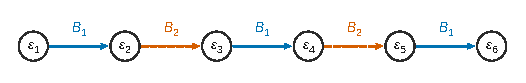
\includegraphics{figures/q20-decomposition-jn.pdf}
\caption*{Figure 2 --- J\_6 vue comme la chaîne ε\_1 → \ldots{} → ε\_6 de la base
canonique : B\_1 (bleu, plein) prend les flèches issues d'un indice
impair, B\_2 (orange, tirets) celles d'un indice pair}
\end{figure}

\hypertarget{question-21}{%
\subsection{Question 21}\label{question-21}}

On a \(V=\sum_{i=1}^{n-2}E_{i+1,i}\) et \(E_C=\sum_{j=1}^{n-1}c_jE_{j,n}\). Posons

\equationajustee{\begin{aligned}
B_1&=\sum_{\substack{1\leqslant i\leqslant n-2\\ i\ \text{impair}}}E_{i+1,i}+\sum_{\substack{1\leqslant j\leqslant n-1\\ j\ \text{pair}}}c_jE_{j,n},\\
B_2&=\sum_{\substack{1\leqslant i\leqslant n-2\\ i\ \text{pair}}}E_{i+1,i}+\sum_{\substack{1\leqslant j\leqslant n-1\\ j\ \text{impair}}}c_jE_{j,n}.
\end{aligned}}

Alors \(B_1+B_2=V+E_C\). Dans \(B_1^2\) interviennent des produits avec \(i,i'\) impairs \(\leqslant n-2\) et \(j,j'\) pairs \(\leqslant n-1\) :

\begin{itemize}
\tightlist
\item
  \(E_{i+1,i}E_{i'+1,i'}=\delta_{i,i'+1}E_{i+1,i'}=0\) (même parité) ;
\item
  \(E_{i+1,i}E_{j,n}=\delta_{i,j}E_{i+1,n}=0\) (parités différentes) ;
\item
  \(E_{j,n}E_{i'+1,i'}=\delta_{n,i'+1}E_{j,i'}=0\) (car \(i'+1\leqslant n-1\)) ;
\item
  \(E_{j,n}E_{j',n}=\delta_{n,j'}E_{j,n}=0\) (car \(j'\leqslant n-1\)).
\end{itemize}

Donc \(B_1^2=0\). De même, en échangeant les parités, \(B_2^2=0\).

\equationajustee{\boxed{\begin{aligned}V+E_C&=B_1+B_2,\\ B_1^2&=B_2^2=0.\end{aligned}}}

\begin{figure}[H]
\centering
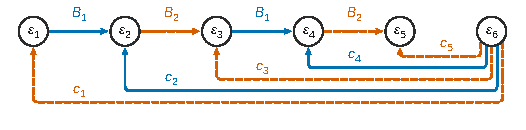
\includegraphics{figures/q21-decomposition-v-ec.pdf}
\caption*{Figure 3 --- V + E\_C pour n = 6 : la chaîne s'arrête en ε\_5, les
retours ε\_6 → ε\_j de poids c\_j vont dans B\_1 si j est pair, dans
B\_2 si j est impair}
\end{figure}

\hypertarget{question-22}{%
\subsection{Question 22}\label{question-22}}

Comme \(v\) n'est pas une homothétie, \(n\geqslant2\). Le corps étant \(\mathbb C\), \(v\) est trigonalisable : soit \((\varepsilon_1,\dots,\varepsilon_n)\) une base de trigonalisation, de matrice \(T\) triangulaire supérieure.

\emph{Cas 1 : \(v\) a deux valeurs propres distinctes \(\lambda\neq\mu\).} Soient \(x\) et \(y\) des vecteurs propres associés. Ils forment une famille libre, et \(P=\operatorname{Vect}(x,y)\) est un plan stable.

Le vecteur \(x+y\), non nul, n'est pas propre. En effet, \(v(x+y)=\lambda x+\mu y=\alpha(x+y)\) imposerait \(\lambda=\alpha=\mu\).

\emph{Cas 2 : \(\operatorname{Sp}(v)=\{\lambda\}\).} La diagonale de \(T\) est constante égale à \(\lambda\). Donc \(N=v-\lambda\,\mathrm{id}\) a une matrice strictement triangulaire supérieure.

Avec \(G_k=\operatorname{Vect}(\varepsilon_1,\dots,\varepsilon_k)\), on a \(N(G_k)\subset G_{k-1}\), d'où \(N^n=0\). Et \(N\neq0\), car \(v\) n'est pas une homothétie.

Soit \(p\geqslant2\) le plus petit entier tel que \(N^p=0\), puis \(y\) tel que \(N^{p-1}(y)\neq0\).

Posons \(x=N^{p-2}(y)\) : on a \(N(x)\neq0\) et \(N^2(x)=0\).

La famille \((x,N(x))\) est libre. Si \(\alpha x+\beta N(x)=0\), appliquer \(N\) donne \(\alpha N(x)=0\), donc \(\alpha=0\), puis \(\beta=0\).

Le plan \(P=\operatorname{Vect}(x,N(x))\) est stable par \(N\), car \(N(N(x))=0\). Il est donc stable par \(v=\lambda\,\mathrm{id}+N\).

Enfin \(x\) n'est pas propre : \(v(x)=\mu x\) donnerait \(N(x)=(\mu-\lambda)x\), ce qui contredit la liberté de \((x,N(x))\).

\equationajustee{\boxed{\text{Il existe un plan stable par }v\text{ contenant un vecteur non nul non propre.}}}

\hypertarget{question-23}{%
\subsection{Question 23}\label{question-23}}

Soit \(M\notin\operatorname{Vect}(I_n)\) et \(v\) l'endomorphisme de \(\mathbb C^n\) canoniquement associé : \(v\) n'est pas une homothétie. Par Q22, soit \(P\) un plan stable et \(x\in P\) non nul et non propre.

La famille \((x,v(x))\) est libre, sinon \(x\) serait propre. Elle est contenue dans \(P\), qui est stable : c'est une base de \(P\).

Complétons-la en une base \(\mathcal B=(x,v(x),f_3,\dots,f_n)\) de \(\mathbb C^n\). Par stabilité de \(P\),

\equationajustee{\operatorname{Mat}_{\mathcal B}(v)=\begin{pmatrix}B&\ast\\(0)&C'\end{pmatrix},\qquad B=\begin{pmatrix}0&b_{1,2}\\1&b_{2,2}\end{pmatrix},}

donc \(b_{2,1}=1\neq0\).

La matrice \(C'\in\mathcal M_{n-2}(\mathbb C)\) est trigonalisable : \(C'=QCQ^{-1}\) avec \(C\) triangulaire supérieure. Avec \(R=\begin{pmatrix}I_2&0\\0&Q\end{pmatrix}\), on obtient

\equationajustee{R^{-1}\begin{pmatrix}B&\ast\\(0)&C'\end{pmatrix}R=\begin{pmatrix}B&\ast Q\\(0)&C\end{pmatrix}.}

Pour \(n=2\), il n'y a pas de bloc \(C\) et la conclusion est déjà acquise.

\equationajustee{\boxed{M\ \text{est semblable \text{à}}\ \begin{pmatrix}B&(?)\\(0)&C\end{pmatrix},\ b_{2,1}\neq0,\ C\ \text{triangulaire \text{supérieure}}.}}

\hypertarget{question-24}{%
\subsection{Question 24}\label{question-24}}

Soit \(M\notin\operatorname{Vect}(I_n)\) ; alors \({}^tM\notin\operatorname{Vect}(I_n)\). Par Q23, \({}^tM=QNQ^{-1}\), où \(N_{i,j}=0\) pour \(i>j\), sauf \(N_{2,1}=b_{2,1}\neq0\).

En transposant, \(M=({}^tQ)^{-1}\,{}^tN\,{}^tQ\) : \(M\) est semblable à \({}^tN\).

Soit \(K=(\delta_{i,n+1-j})\) la matrice de permutation qui renverse l'ordre de la base. Elle vérifie \(K^2=I_n\) et \((KSK)_{i,j}=S_{n+1-i,n+1-j}\) pour toute \(S\).

Posons \(A'=K\,{}^tN\,K\), semblable à \(M\). Alors

\equationajustee{A'_{i,j}=({}^tN)_{n+1-i,\,n+1-j}=N_{n+1-j,\,n+1-i}.}

Si \(i>j\), on a \(n+1-j>n+1-i\) : ce coefficient de \(N\) est strictement sous la diagonale, donc nul. L'exception est \((n+1-j,n+1-i)=(2,1)\), c'est-à-dire \((i,j)=(n,n-1)\), où il vaut \(b_{2,1}\neq0\).

\equationajustee{\boxed{\text{Toute matrice de }\mathcal M_n(\mathbb C)\setminus\operatorname{Vect}(I_n)\text{ est semblable \text{à} une matrice presque triangulaire \text{supérieure}.}}}

\hypertarget{question-25}{%
\subsection{Question 25}\label{question-25}}

Soit \(n=\dim E\) et \(u\) de trace nulle.

\emph{Cas où \(u\) est une homothétie} (en particulier si \(n\leqslant1\)). On écrit \(u=\lambda\,{\mathrm{id}}_E\), et \(\operatorname{tr}u=n\lambda=0\).

Donc \(u=0=0+0+0+0\), élément de \(\Sigma_4\mathcal C(E)\) ; si \(n=0\), \(u=0\) aussi.

\emph{Cas général} : \(n\geqslant2\) et \(u\) n'est pas une homothétie. Soit \(A\) la matrice de \(u\) dans une base \(\mathcal B\) ; on a \(A\notin\operatorname{Vect}(I_n)\).

\begin{itemize}
\tightlist
\item
  Par Q24, \(A=RA'R^{-1}\), avec \(A'\) presque triangulaire supérieure et \(\operatorname{tr}A'=\operatorname{tr}A=0\).
\item
  Par Q19, il existe \(C_0\) et \(Q\in GL_n(\mathbb C)\) tels que \(A'+V+E_{C_0}=QJ_nQ^{-1}\).
\item
  Par Q20, \(J_n=D_1+D_2\) avec \(D_1^2=D_2^2=0\).
\item
  Par Q21, \(V+E_{C_0}=B_1+B_2\) avec \(B_1^2=B_2^2=0\).
\end{itemize}

Donc

\equationajustee{A'=QD_1Q^{-1}+QD_2Q^{-1}+(-B_1)+(-B_2).}

C'est une somme de quatre matrices de carré nul, car \((QDQ^{-1})^2=QD^2Q^{-1}\) et \((-B)^2=B^2\).

En conjuguant par \(R\), \(A\) est somme de quatre matrices de carré nul. Par l'isomorphisme linéaire \(v\mapsto\operatorname{Mat}_{\mathcal B}(v)\), qui transforme une composée en produit, \(u\) est somme de quatre endomorphismes de carré nul.

\equationajustee{\boxed{\operatorname{tr}(u)=0\ \Longrightarrow\ u\in\Sigma_4\mathcal C(E).}}

Avec Q8, \(\Sigma_4\mathcal C(E)=\Sigma_\infty\mathcal C(E)=\mathcal H(E)\). La partie C montre que \(4\) ne peut pas être remplacé par \(3\) dès que \(\dim E\geqslant5\).

\end{document}
